\insertdesignoverview{Drivetrain}
{Create a stable drivetrain that can scale the crater to recover minerals quickly and effectively} % Goals of the mechanism
{10-12.JPG}% CAD Image
{drivetrain_1.JPG}% Build Image
{0.25" Medium Density Fiberboard, Aluminum, ABS Plastic, Steel, Retaining Rings}% Materials ex. 0.25" MDF, Aluminum, etc
{Laser Cutting, 3D Printing, CNC Milling, Lathe}% Manufacturing Processes ex. Laser Cut, 3D print, etc.

\subsection*{How it Works}
The drivetrain is composed of two modules connected by a center chassis where the motors are built on. Each module has two 20:1 BaneBots planetary gearboxes which spin a driver gear. This gear is meshed in a 1:4 ratio to the gear attached to each wheel. Each 16" wheel has a notch cut in it to allow us to go over the crater. The wheel assemblies ride on bearings that are fixed onto custom 3D printed pieces in the wood.

\begin{figure}[htp]
\centering
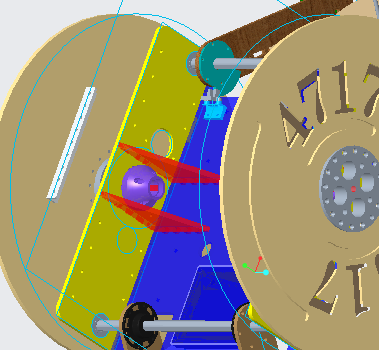
\includegraphics[width=.8\linewidth]{Design_Overview/DT_cad.PNG}
\caption{Another look at the CAD of our Drivetrain}
\label{fig:iteration}
\end{figure}

\subsection*{Iterations}
In prior years, our team utilized belts and pulleys to power our drive train. We found that for this game, going over the crater is essential and bigger wheels would make that task much easier than having a low profile drive train with belts and pulleys. Our first prototype consisted of four 40:1 motors with a 40T driver gear actuating a 120T gear on the output shaft. However, given that the stabilization arms required another two motors, we tried something new by only using one motor to power each side. This worked fairly well for the team, as we didn't compromise on speed or efficiency. In addition, we had to make some changes to provide some horizontal support. 

\subsection*{Mechanism Accomplishments}
\begin{itemize}
    \item It can drive up the crater
    \item It can quickly traverse the field, going from the crater to the lander
    \item Its design allows for more space to add more components
\end{itemize} 

